\chapter{Implémentation}
        \section{Choix des technologies} 
        \paragraph{} 
\begin{tabular}{|c|p{1.5cm}|p{2.7cm}|p{4cm}|}
        \hline
        Technologie & Version & Utilité & Raison du choix \\
        \hline
        Linux & Ubuntu 20.04.1 LTS & OS & Les trois membres utilisent Linux \\
        \hline
        Git/Github & 2.25.1 & Système de contrôle de version & Il permet de travailler à distance et en même temps et de garder une trace des différentes versions\\
        \hline 
        StarUml & 4.0.0 & Conception & Le choix de UML a été imposé par le client dès le départ. \\
        \hline 
        MySQL & 15.1 & SGBD & Open source | Facile à utiliser\\
        \hline 
        MySQL Workbench & 8.0 & Modélisation des données & Open source | Design Database sans code\\
        \hline
        PHP & 7.4.13 & Codage backend & Open source | Robuste | Sécurité | Imposé par le client\\
        \hline
\end{tabular}
\begin{tabular}{|c|p{1.5cm}|p{2.7cm}|p{4cm}|}
        \hline
        Laravel Framework & 8.15.0 & Programmation web & Prise en charge de l’architecture MVC | Facilite d’utilisation du Framework | Sécurité et performance | Documentation et communauté\\
        \hline
        HTML5 & 5 & Programmation structure frontend & Open source | Facilité\\
        \hline
        CSS3 & 3 & Programmation design frontend & Open source | Facilité\\
        \hline
        Bootstrap & 3.3.7 & Programmation design frontend & Open source | Facilité\\
        \hline
        Jquery & 3.1.2 & Programmation gestion des evenements frontend & Open source | Facilité\\
        \hline
        Google: Gmail API &  & SMTP & Server mail pour délivrer les email\\
        \hline
\end{tabular}

\section{La hiérarchie dans l'application}
\paragraph{}
Trois niveaux d'utilisation sont considérés au sein de l'application.
Chacun d'eux détient des privilèges en plus de celui qui vient directement après lui.
Les abonnés sont ceux qui peuvent poser le moins d'actions possibles dans le système. ils 
ne peuvent rien faire de plus que lire les données disponibles. De ce fait, 
ils peuvent voir tous les livres qui sont disponibles à chaque instant, et recevoir 
des notifications lorsqu'ils auront passé trop de temps avec un ouvrage en main.\par 
De leur côté, les bibliothécaires détiennent des droits de ressources matérielles. En plus
des droits d'accès des abonnés, ils peuvent agir sur les différents 
emprunts ainsi que que sur les données relatives aux ouvrages. \par 
Et enfin, le gestionnaire peut tout faire, et plus particulièrement gérer les 
utilisateurs du système.
\section{Interface utilisateur}
\paragraph{}       
L'interface utilisateur a été réfléchi de telle sorte que n'importe qui 
peut se retrouver facilement sur l'application. Aucun téléchargement préalable n'est requis, de même 
qu'il ne sera pas du tout nécessaire de faire un cours complet pour expliquer à un nouvel utilisateur
les différentes utilités de chaque bouton.

\section{Diagrammes}
\subsection{Diagrammes des cas d'utilisation}
\subsubsection{Cas d'utilisation général} 
\begin{figure}[h]
        \centering
        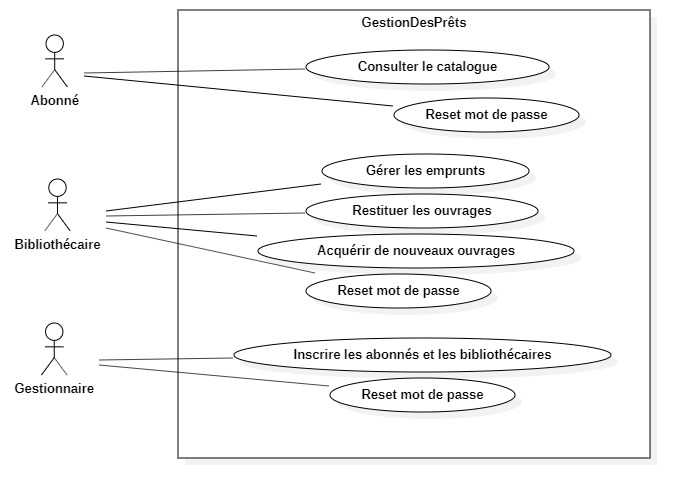
\includegraphics[width=1\textwidth]{generalUseCase}
        \caption{Diagramme des cas d'utilisation général}
        \label{image-generalUseCase}
        \end{figure}
\paragraph{}
Lorem ipsum dolor sit amet, consectetur adipiscing elit. Mauris at ultrices purus. Donec finibus metus et augue sodales posuere. Proin sit amet turpis dictum, iaculis felis in, scelerisque massa. Nullam aliquam nunc eget fringilla volutpat. Integer et mauris et massa imperdiet scelerisque mollis at sapien. Donec condimentum felis eget sagittis ultricies. Nunc laoreet augue id consectetur vulputate. Cras sagittis aliquam risus sit amet tempus. Curabitur finibus neque eget magna efficitur, sed dignissim quam sagittis. Ut euismod justo id gravida pulvinar. Ut urna magna, auctor maximus volutpat ac, elementum sed mi.

\subsubsection{Consultation du catalogue} 
\begin{figure}[h]
        \centering
        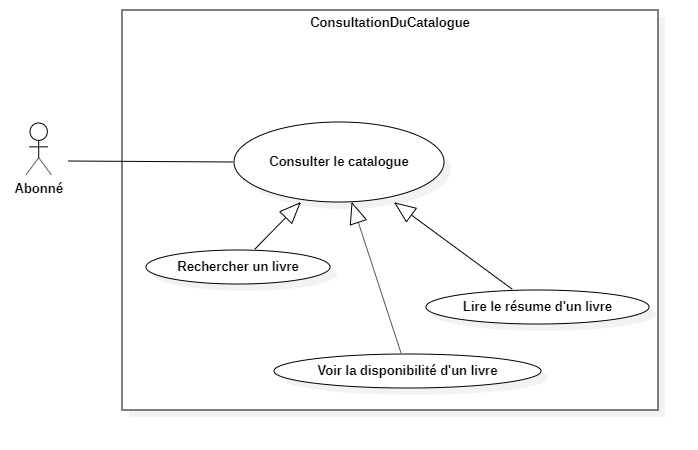
\includegraphics[width=1\textwidth]{consultationDuCatalogueUseCase}
        \caption{Diagramme du cas de consultation du catalogue}
        \label{image-consultationDuCatalogueUseCase}
        \end{figure}
\paragraph{}
Lorem ipsum dolor sit amet, consectetur adipiscing elit. Mauris at ultrices purus. Donec finibus metus et augue sodales posuere. Proin sit amet turpis dictum, iaculis felis in, scelerisque massa. Nullam aliquam nunc eget fringilla volutpat. Integer et mauris et massa imperdiet scelerisque mollis at sapien. Donec condimentum felis eget sagittis ultricies. Nunc laoreet augue id consectetur vulputate. Cras sagittis aliquam risus sit amet tempus. Curabitur finibus neque eget magna efficitur, sed dignissim quam sagittis. Ut euismod justo id gravida pulvinar. Ut urna magna, auctor maximus volutpat ac, elementum sed mi.

\subsubsection{Acquisition des ouvrages} 
\begin{figure}[h]
        \centering
        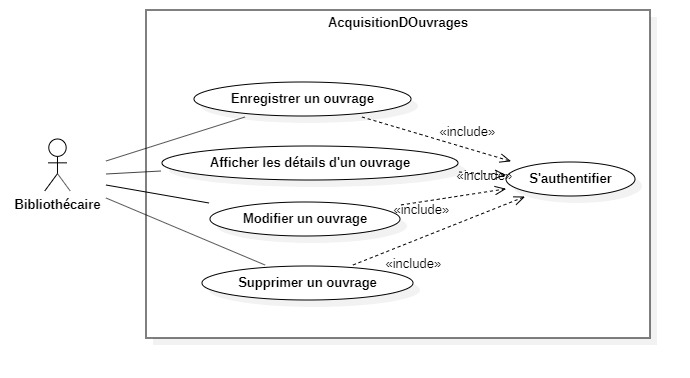
\includegraphics[width=1\textwidth]{acquisitionDesOuvragesUseCase}
        \caption{Diagramme du cas d'acquisition des ouvrages}
        \label{image-acquisitionDesOuvragesUseCase}
        \end{figure}
\paragraph{}
Lorem ipsum dolor sit amet, consectetur adipiscing elit. Mauris at ultrices purus. Donec finibus metus et augue sodales posuere. Proin sit amet turpis dictum, iaculis felis in, scelerisque massa. Nullam aliquam nunc eget fringilla volutpat. Integer et mauris et massa imperdiet scelerisque mollis at sapien. Donec condimentum felis eget sagittis ultricies. Nunc laoreet augue id consectetur vulputate. Cras sagittis aliquam risus sit amet tempus. Curabitur finibus neque eget magna efficitur, sed dignissim quam sagittis. Ut euismod justo id gravida pulvinar. Ut urna magna, auctor maximus volutpat ac, elementum sed mi.

\subsubsection{Gestion des emprunts} 
\begin{figure}[ht]
        \centering
        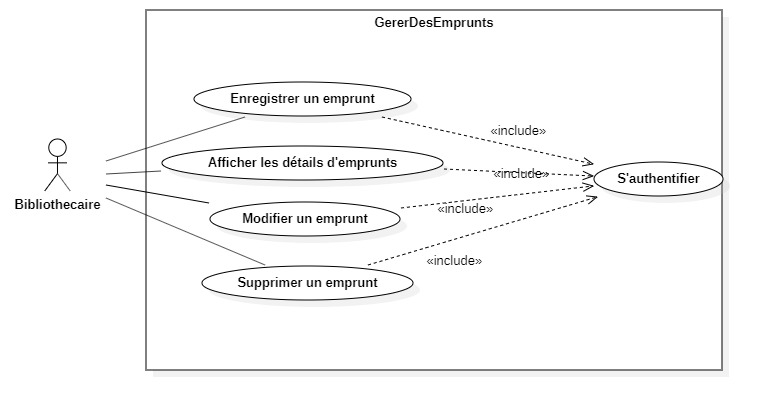
\includegraphics[width=1\textwidth]{gestionDesEmpruntsUseCase}
        \caption{Diagramme du cas de gestion des emprunts}
        \label{image-gestionDesEmpruntsUseCase}
        \end{figure}
\paragraph{}
Lorem ipsum dolor sit amet, consectetur adipiscing elit. Mauris at ultrices purus. Donec finibus metus et augue sodales posuere. Proin sit amet turpis dictum, iaculis felis in, scelerisque massa. Nullam aliquam nunc eget fringilla volutpat. Integer et mauris et massa imperdiet scelerisque mollis at sapien. Donec condimentum felis eget sagittis ultricies. Nunc laoreet augue id consectetur vulputate. Cras sagittis aliquam risus sit amet tempus. Curabitur finibus neque eget magna efficitur, sed dignissim quam sagittis. Ut euismod justo id gravida pulvinar. Ut urna magna, auctor maximus volutpat ac, elementum sed mi.

\subsubsection{Restitution des ouvrages} 
\begin{figure}[h]
        \centering
        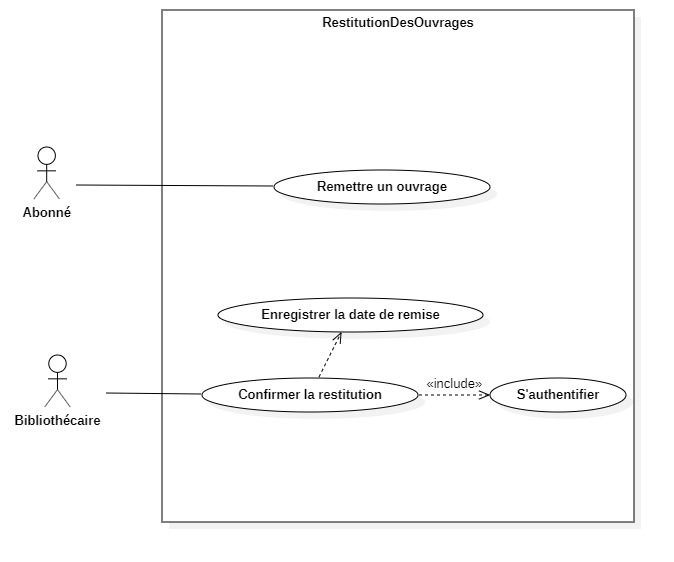
\includegraphics[width=1\textwidth]{restitutionDesOuvragesUseCase}
        \caption{Diagramme du cas de restitution des ouvrages}
        \label{image-restitutionDesOuvragesUseCase}
        \end{figure}
\paragraph{}
Lorem ipsum dolor sit amet, consectetur adipiscing elit. Mauris at ultrices purus. Donec finibus metus et augue sodales posuere. Proin sit amet turpis dictum, iaculis felis in, scelerisque massa. Nullam aliquam nunc eget fringilla volutpat. Integer et mauris et massa imperdiet scelerisque mollis at sapien. Donec condimentum felis eget sagittis ultricies. Nunc laoreet augue id consectetur vulputate. Cras sagittis aliquam risus sit amet tempus. Curabitur finibus neque eget magna efficitur, sed dignissim quam sagittis. Ut euismod justo id gravida pulvinar. Ut urna magna, auctor maximus volutpat ac, elementum sed mi.

\subsubsection{Gestion des utilisateurs} 
\begin{figure}[h]
        \centering
        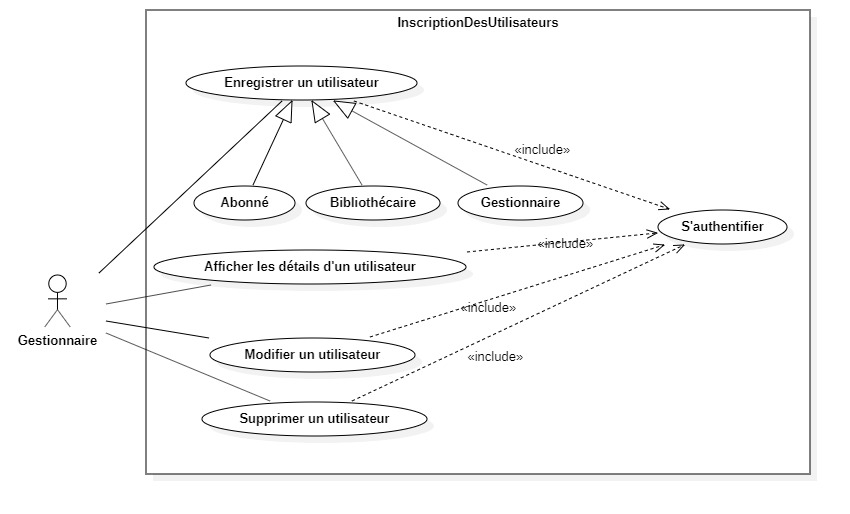
\includegraphics[width=1\textwidth]{gestionDesUtilisateursUseCase}
        \caption{Diagramme du cas de gestion des utilisateurs}
        \label{image-gestionDesUtilisateursUseCase}
        \end{figure}
\paragraph{}
Lorem ipsum dolor sit amet, consectetur adipiscing elit. Mauris at ultrices purus. Donec finibus metus et augue sodales posuere. Proin sit amet turpis dictum, iaculis felis in, scelerisque massa. Nullam aliquam nunc eget fringilla volutpat. Integer et mauris et massa imperdiet scelerisque mollis at sapien. Donec condimentum felis eget sagittis ultricies. Nunc laoreet augue id consectetur vulputate. Cras sagittis aliquam risus sit amet tempus. Curabitur finibus neque eget magna efficitur, sed dignissim quam sagittis. Ut euismod justo id gravida pulvinar. Ut urna magna, auctor maximus volutpat ac, elementum sed mi.



\subsection{Diagrammes de séquence}
\paragraph{} 
Lorem ipsum dolor sit amet, consectetur adipiscing elit. Mauris at ultrices purus. Donec finibus metus et augue sodales posuere. Proin sit amet turpis dictum, iaculis felis in, scelerisque massa. Nullam aliquam nunc eget fringilla volutpat. Integer et mauris et massa imperdiet scelerisque mollis at sapien. Donec condimentum felis eget sagittis ultricies. Nunc laoreet augue id consectetur vulputate. Cras sagittis aliquam risus sit amet tempus. Curabitur finibus neque eget magna efficitur, sed dignissim quam sagittis. Ut euismod justo id gravida pulvinar. Ut urna magna, auctor maximus volutpat ac, elementum sed mi.
\subsection{Diagrammes de ce ce qu'on a demande}
\paragraph{} 
Lorem ipsum dolor sit amet, consectetur adipiscing elit. Mauris at ultrices purus. Donec finibus metus et augue sodales posuere. Proin sit amet turpis dictum, iaculis felis in, scelerisque massa. Nullam aliquam nunc eget fringilla volutpat. Integer et mauris et massa imperdiet scelerisque mollis at sapien. Donec condimentum felis eget sagittis ultricies. Nunc laoreet augue id consectetur vulputate. Cras sagittis aliquam risus sit amet tempus. Curabitur finibus neque eget magna efficitur, sed dignissim quam sagittis. Ut euismod justo id gravida pulvinar. Ut urna magna, auctor maximus volutpat ac, elementum sed mi.
\subsection{Diagrammes de ce qu'on n'a pas demande}
\paragraph{} 
Lorem ipsum dolor sit amet, consectetur adipiscing elit. Mauris at ultrices purus. Donec finibus metus et augue sodales posuere. Proin sit amet turpis dictum, iaculis felis in, scelerisque massa. Nullam aliquam nunc eget fringilla volutpat. Integer et mauris et massa imperdiet scelerisque mollis at sapien. Donec condimentum felis eget sagittis ultricies. Nunc laoreet augue id consectetur vulputate. Cras sagittis aliquam risus sit amet tempus. Curabitur finibus neque eget magna efficitur, sed dignissim quam sagittis. Ut euismod justo id gravida pulvinar. Ut urna magna, auctor maximus volutpat ac, elementum sed mi.
